\section{Einführung in Deepfakes}
\subsection{Definition}
Der Begriff Deepfake setzt sich aus den englischen Begriffen Deep Learning und Fake zusammen. Hierbei steht Deep Learning für eine Methode des maschinellen Lernens und Fake für eine Fälschung.\newline
"Bei Deepfakes handelt es sich um einen Teilbereich synthetischer audiovisueller Medien: die Manipulation oder auch synthetische Erzeugung von Abbildungen, Videos und/oder Audiospuren menschlicher Gesichter, Körper oder Stimmen, zumeist mithilfe von KI."\cite{SpringerLink}
\cite{SpringerLink}
\newline
Deepfakes werden mit Hilfe von künstlicher Intelligenz und Deep Learning Technologien erstellt, um Personen realistische Handlungen ausführen oder Worte sagen zu lassen, in Form von Video, Bild oder Audio. Es handelt sich hierbei um gefälschte Darstellungen, die möglichst realitätsnah dargestellt werden.\cite{ScienceDirect}

\subsection{Hintergrund}
Deepfake ist eine Manipulationstechnik, die es Benutzern ermöglicht, das Gesicht einer Person mit einer anderen Person auszutauschen. Eine optimale Manipulation wird durch Verwendung mehreren Hunderten oder Tausenden Fotos der Zielperson erreicht. Das führt dazu, dass oft prominete Personen als Zielperson gewählt werden, da von ihnen viele Bilder im Internet existieren.\newline
Bild- und Videomanipulationstechnologien bauen auf Techniken aus dem Bereich der künstlichen Intelligenz auf, welcher das Ziel verfolgt, menschliche Denkprozesse und Verhaltensweisen zu verstehen.
Da maschinelles Lernen einem System ermöglicht aus Daten zu lernen, ist diese Technik wichtig für das erstellen von Deepfakes. \newline
Deepfakes sind aus zwei Gründen beliebt: erstens wegen der Fähigkeit aus Daten wie Fotos und Videos, realistische Ergebnisse erzeugen zu können und zweitens die Verfügbarkeit der Technik, da diese für jeden leicht zu erreichen und durchzuführen ist.
Es gibt Apps, welche die Schritte des Deepfakes-Algorithmus erklärt und so Personen mit wenig Kenntnissen über maschinelles Lernen oder Programmierung die Möglichkeit bietet ein Deepfake Bild oder Video zu erstellen. \newline
Das führt zu einem Problem der heutigen Gesellschaft, da Deepfakes hauptsächlich aus Rache, Erpressung einer Person oder Verbreitung von Fake News einer höheren Person (bspw. eines Politikers) ausgenutzt werden.\cite{Jatit}

\subsubsection*{Geschichte}
Das Manipulieren von Bildern wurde nicht erst in den letzten Jahren bekannt. Denn auch schon früher wurden Bilder zum Beispiel von Hitler, Stalin, oder Breschnew manipuliert, um so die Geschichte zu ihren Gunsten verändern zu können.
Damals erforderte es allerdings deutlich mehr Zeit und kompliziertere Techniken während der Fotoentwicklung in der Dunkelkammer, um ein Bild zu verfälschen. Doch durch die schnelle Entwicklung der Technologien wurde der Prozess ein Bild zu manipulieren zunehmend schneller.
Anfangs begannen ausschließlich Forscher der 1990er Jahre die Entwicklung der Deepfake-Technologie zu übernehmen, diese wurde jedoch später von Amateuren in den Online-Communities unterstützt.
Die Akademiker Christoph Bregler, Michele Covell und Malcolm Slaney entwickelten 1997 ein Programm, welches vorhandenes Videomaterial einer sprechenden Person anpassen konnte, dass diese Person die Wörter von einer anderen Audiospur nachahmte.
Das Programm baut auf einer älteren Technologie auf, welches bereits Gesichter interpretieren, Audio aus Texten synthetisieren und Lippen im 3D-Raum modellieren konnte.
Jedoch war dieses entwickelte Programm von den drei Akademikern das erste, welches alle Komponenten zusammenfügen und überzeugend animieren konnte. So war es möglich eine neue Gesichtsanimation aus einer Audioausgabe zusammenstellen zu können.\newline
Zu Beginn der 2000er Jahre wurde die Entwicklung der Gesichtserkennung mit dem Computer immer weiter vorangetrieben,
sodass es zu großen Verbesserungen der Technologie wie \glspl{motiontracking} kam, welche die heutigen Deepfakes so
überzeugend machen.\newline
In den Jahren 2016 und 2017 gab es zwei Projekt Veröffentlichungen. Einmal das Face2Face-Projekt der Technischen Universität München und einmal das Synthesizing Obama-Projekt der University of Washington. \newline
Das Face2Face Projekt versucht Echtzeitanimationen zu erstellen, indem es den Mundbereich des Zielvideos durch einen Schauspieler ersetzt, während das Synthesizing Obama-Projekt sich damit beschäftigte Videomaterial des ehemaligen Präsidenten Barack Obama zu modifizieren.\cite{ResearchGate}\newline
Im Jahr 2017 wurde das gefälschte Video des ehemaligen US-Präsidenten Barack Obama veröffentlicht und soll als Warnung der Technologie und deren potenziellen Auswirkungen gelten.
Ende 2017 veröffentlichte ein Nutzer auf einer Webseite names Reddit pornografische Inhalte und behauptete, dass diese zu bekannten Personen wie zum Beispiel Taylor Swift oder Scarlett Johansson gehören.
Auch wenn diese Bilder und Videos schnell wieder gelöscht wurden, erregte diese auf Deep Learning basierende Gesichtsersatztechnik die Aufmerksamkeit der Medien und verbreitete sich in vielen Internetforen.
Alle Inhalte, die mit der Deepfake Technik zu tun hatten, wurden am 7. Februar 2018 auf fast allen Internetforen entfernt und verboten.
Trotz des Verbots hat sich die Technik dennoch weiterhin durchgesetzt und wurde weltweit verbreitet.
Bei der Person, die die Deepfake-Technik entwickelt hat, soll es sich um einen Software-Ingenieur handeln, der ein Entwicklungs-Kit herausbrachte, mit dem es einem Benutzer selbst ermöglicht, eigene manipulierte Bilder oder Videos zu erstellen.
Durch die Hilfe von Open Source Tools und Funktionen von großen Softwareunternehmen wie NVidia und Google wurde die Deepfake-Technike entwickelt. Was bedeutet, dass für die Entwicklung technisches Wissen und Verständnis erforderlich sind, jedoch der Großteil der Software schon zuvor in der Öffentlichkeit zur Verfügung stand.
Als klar wurde, dass selbst eine Person ohne viel Wissen in dem Gebiet, beliebig viele visuelle Medien manupulieren kann, wurde die Bedrohung der Deepfake-Technik ernst und das US-Verteidigungsministerium stellte sich ein.
Auch im Jahr 2018 wurde ein Deepfake Video von damaligen Präsidenten Donald Trump in den Medien hochgeladen, in dem die Belgier aufgefordert wurden, aus dem Pariser Klimaschutzabkommen auszusteigen.\newline
Durch solche Veröffentlichungen der Deepfake Videos zeigte sich, dass die Technologie sich schnell weiterentwickelt und in der Lage ist einen großen Teil der Öffentlichkeit in die Irre führen zu können.\cite{Jatit}

\subsection{Theoretische Grundlagen}
Wie in fast allen Modellen der künstlichen Intelligenz, wird auch bei den Deepfakes Ausgangsmaterial benötigt. Das kann zum Beispiel Videomaterial oder Bilder von Personen sein, die man manipulieren möchte. Auch hier gilt je mehr Ausgangsmaterial vorhanden ist, desto besser erfolgt das Training des Modells. Bei einer Video Manipulation wird das Ergebnis besser, je mehr Videomaterial aus verschiedenen Perspektiven und verschiedenen Mimiken vorhanden ist.\cite{HochschuleDerMedien}\newline
\subsubsection{Autoencoder}
Ein Ansatz zur Erstellung von Deepfakes ist die Autoencoder Variante. Dieses neuronale Netzerzeugt aus einem Eingabebild ein digitales Abbild (Encoding), indem es durch ein Verfahren wie \gls{MaxPooling} verkleinert und auf wesentliche Kernmerkale des Bildes reduziert. Das encodierte Bild wird dann im Anschluss versucht, dass Bild möglichst orginalgetreu nachzubilden (Decoding). Das Ziel des Decoding ist es also, ein identisches, künstliches Abbild des encodierten Eingabebildes zu erzeugen. Um die Robustheit des Autoencoders zu erhöhen, ist es ratsam die Eingabebilder zu verzerren, Auflösung zu variieren und die Größe zu verändern.  Über längere Zeit des Trainings wird das Netz immer präziser, sodass der Unterschied zwischen Eingabngs- und Ausgangsbild nahezu nicht mehr vorhanden ist.\newline
Um zwei Personen zu tauschen, wird das Autoencoder Verfahren auf beide Personen angewendet. Der Encoder bleibt hier der gleiche für beide Personen und für den Decoder gibt es 2 verschiedene. Während des Trainings des Deepfakes wird zunächst das Bildmaterial von Person A encodiert und anschließend mit Decoder A nachgestellt. Danach folgt dasselbe Training mit Person B und Decoder B. Nach dem Training beider Personen wird der Decoder A durch den Decoder B ersetzt, wodurch dann der Deepfake entsteht.\cite{HochschuleDerMedien}
\begin{figure}[H]
    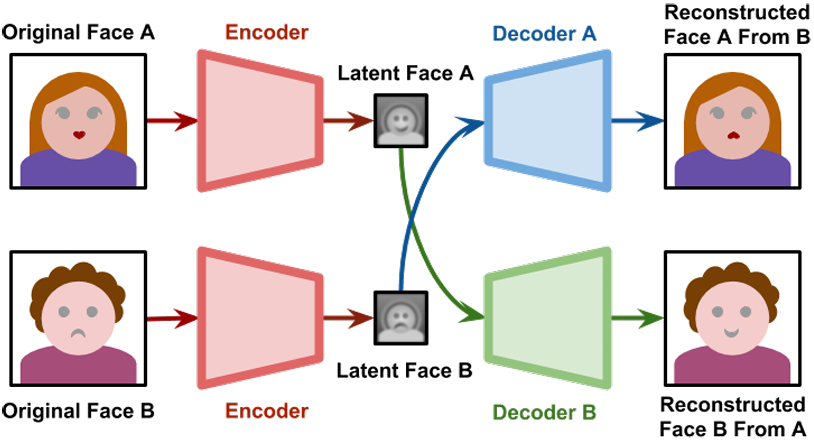
\includegraphics[width=0.7\textwidth]{Bilder/Autoencoder}
    \centering
    \caption{Darstellung des Autoencoders zur Erstellung eines Deepfakes\cite{HochschuleDerMedien}}
    \label{fig:Autoencoder}
\end{figure}

\begin{itemize}
    \item \textbf{Funktion des Autoencoder:} \\
    Autoencoder entdecken latente Variablen. Hierfür leiten sie die Eingabedaten durch einen Engpass (Code), bevor sie den Decoder erreichen. Dieser Engpass zwingt den Encoder zu lernen, dass nur die Informationen extrahiert und weitergeleitet werden, die für eine präzise Rekonstruktion der ursprünglichen Eingabe am nützlichsten sind.\newline
    Der Encoder umfasst hierbei mehrere Schichten, welche eine komprimierte Darstellung der Eingabedaten durch Dimensionreduktion erzeugen. In einem typischen Autoencoder reduzieren die verborgenen Schichten die Anzahl der Knoten schrittweise im Vergleich zur Eingabeschicht. Während die Daten die Encoderschichten durchlaufen, werden sie durch einen Prozess (Strauchung) in weniger Dimensionen komprimiert.\newline
    Der Engpass (auch Code genannt) besitzt die stärkste komprimierte Darstellung der Eingabe. Er wird sowohl als Ausgangsschicht des Encodernetzes als auch die Eingabeschicht des Decodernetzes betrachtet. Eines der Ziele des Entwurfs und Trainings eines Autoencoders besteht darin, die kleinstmögliche Anzahl der relevantesten Merkmale zu ermitteln, welche für eine effektive Rekonstruktion der Eingabedaten erforderlich sind. Der austretende Code (Latent-Raum-Darstellung) dieser Schicht, wird in dem Decoder weitergeleitet und dort weiter verarbeitet.\newline
    Der Decoder besteht aus verborgenen Schichten, von dem die Anzahl der Knoten zunehmend wächst, um so die codierte Darstellung der Daten zu decodieren und in die ursprüngliche Form vor der Codierung wiederherzustellen. Die rekonstruierte Ausgabe wird mit der "Ground Truth", in den meisten Fällen die ursprünglichen Eingabe, verglichen, um die Wirksamkeit des Autoencoders zu bewerten.\newline
    In vielen Anwendungen von Autoencodern kann der Decoder nach dem Training gelöscht werden, da in solchen Fällen der Decoder nur dazu da war den Encoder zu trainieren. In einem \gls{gan} ist dieser Vorgang zu vergleichen mit der Rolle des Diskriminators, welcher dann als Komponente eines anderen neuronalen Netzes verwendet wird. Jedoch erfüllt der Decoder in vielen Autoencodern nach dem Training weiterhin einen Zweck, wie zum Beispiel das Ausgeben neuer Datenproben in \gls{VAE}s.\cite{ibmAutoencoder}
\end{itemize}

\subsubsection{Generative Adversarial Networks (GANs)}\label{subsubsec:gans}

Mit dem Aufkommen von \glspl{gan} hat sich die Erstellung von Deepfakes erheblich vereinfacht und verbessert.
\glspl{gan} bestehen aus zwei neuronalen Netzwerken, einem Generator und einem Diskriminator, die gegeneinander trainiert werden.\cite{Deepfakes-a-survey-and-introduction-to-the-topical-collection}

\textbf{Technische Details:}
\begin{itemize}
    \item Der \textbf{Generator} erzeugt Bilder, die versuchen, echte Bilder nachzuahmen.
    \item Der \textbf{Diskriminator} bewertet die Bilder des Generators und unterscheidet zwischen echten und generierten Bildern.
    \item Durch diesen Wettbewerb verbessert sich die Qualität der erzeugten Bilder stetig.
\end{itemize}

\textbf{Vor- und Nachteile:}
\begin{itemize}
    \item \textbf{Vorteile:} Hohe Qualität der erzeugten Bilder, Möglichkeit zur Erstellung realistischer und dynamischer Gesichtsausdrücke.
    \item \textbf{Nachteile:} Erfordert große Datenmengen und Rechenressourcen für das Training, anfällig für Artefakte und Unstimmigkeiten bei komplexen Bewegungen \cite{Deepfakes-An-Overview}.
\end{itemize}

\textbf{Einsatz im Kontext von Social Engineering:} \gls{gan}-basierte Deepfakes sind effektiver und leichter zu erstellen, was sie zu einem mächtigen Werkzeug für Angreifer im Bereich Social Engineering macht.
Sie können verwendet werden, um gefälschte Videos zu erstellen, die Vertrauen erwecken und die Opfer täuschen.
Um ein Modell zu trainieren werden mehrere Minuten Video-Material der Zielperson und viel Rechenleistung benötigt.
Ist das Modell dann trainiert, können je nach Auflösung Videos \gls{jit}, auch auf einem schwächeren PC, manipuliert werden.
\glspl{gan} sind heutzutage nach wie vor \gls{sota} und machen den Großteil der erstellten Deepfakes aus.
Auch \gls{dfl} basiert auf dieser Technik und macht laut Entwickler ca. $95\%$ der im Internet kursierenden Deepfakes aus\cite{dfl-github-repo}.

\subsubsection{FSGAN und FSGANv2}\label{subsubsec:fsgan}

Eine Weiterentwicklung der \gls{gan}-Technologie sind die Face Swapping \glspl{gan} (\gls{fsgan}) und ihre verbesserte Version, FSGANv2.
Diese Technologien sind speziell für den Gesichtstausch und die Gesichtsnachstellung entwickelt worden.

\textbf{Technische Details:}
\begin{itemize}
    \item \gls{fsgan} nutzt \glspl{gan}, um Gesichtszüge von einer Quelle auf ein Zielvideo zu übertragen, ohne dass eine explizite 3D-Modellierung erforderlich ist.
    \item FSGANv2 verbessert diese Methode durch bessere Algorithmen zur Anpassung der Gesichtsausdrücke und -bewegungen sowie durch die Verwendung von fortschrittlichen Netzwerktechniken, um die Konsistenz und Realismus zu erhöhen \cite{fsganv2}.
\end{itemize}

\textbf{Vor- und Nachteile:}
\begin{itemize}
    \item \textbf{Vorteile:} Sehr realistische Ergebnisse, weniger Training und Daten erforderlich im Vergleich zu reinen \glspl{gan}, bessere Anpassung an unterschiedliche Gesichtsausdrücke und Beleuchtungen.
    \item \textbf{Nachteile:} Trotz Verbesserungen immer noch anfällig für subtile Unstimmigkeiten, die bei genauer Betrachtung auffallen können \cite{face-swapping-and-reenactment}.
\end{itemize}

\textbf{Einsatz im Kontext von Social Engineering:} \gls{fsgan} und FSGANv2 sind äußerst effektiv für Social Engineering-Angriffe, da sie schon mit wenigen Ausgangsbildern realistische Deepfakes erstellen können.
Sie können verwendet werden, um falsche Identitäten zu erstellen und Vertrauen zu gewinnen, was das Risiko und den potenziellen Schaden solcher Angriffe erhöht \cite{deepfacelab}.

\subsubsection{Gemeinsamkeiten und Unterschiede}\label{subsubsec:gemeinsamkeiten-unterschiede}

\textbf{Gemeinsamkeiten:}
\begin{itemize}
    \item Alle Methoden zielen darauf ab, realistische Fälschungen zu erstellen, die schwer zu erkennen sind.
    \item Nutzung von KI und maschinellem Lernen zur Verbesserung der Qualität und Realismus der erzeugten Videos.
\end{itemize}

\textbf{Unterschiede:}
\begin{itemize}
    \item 3D-Modellierung erfordert manuelle Arbeit, ist weniger flexibel und kann nicht in Echtzeit realisiert werden.
    \item \glspl{gan} und deren Weiterentwicklungen (\gls{fsgan}, FSGANv2) bieten automatisierte Lösungen mit höherer Qualität und Flexibilität.
    \item \gls{fsgan} und FSGANv2 sind speziell auf Gesichtsmanipulation optimiert und bieten bessere Ergebnisse bei der Anpassung an verschiedene Bedingungen\cite{Deepfakes-a-survey-and-introduction-to-the-topical-collection}.
\end{itemize}

Insgesamt zeigt sich, dass die Weiterentwicklung der Deepfake-Technologien, insbesondere durch \glspl{gan} und deren Spezialisierungen wie \gls{fsgan} und FSGANv2, erheblich zur Verbesserung der Qualität und Realismus beigetragen hat.
Dies stellt jedoch auch eine größere Bedrohung im Bereich des Social Engineering dar, da die Täuschungsabsicht hinter den erzeugten Medieninhalten immer schwerer zu durchschauen ist.

\subsection{Arten von Deepfakes}
Deepfakes können in drei Hauptarten unterteilt werden: Video Deepfakes, Audio Deepfakes und Foto Deepfakes. Diese drei Arten lassen sich zusätzlich auch noch miteinander kombinieren.\cite{ResearchGate}\newline
\subsubsection*{Video Deepfakes}
Bei Video Deepfakes wird zusätzlich zwischen 3 Arten der Manipulation unterschieden. Auf welche Art der Manipulation zurückgegriffen wird, ist davon abhängig, was der Hauptgrund der Nutzung eines Video Deepfakes ist.\cite{ResearchGate}

\subsubsection*{Face Swapping}
Eine der Arten ist das Face Swapping, bei dem die Gesichter auf Bildern oder Videos durch Fake Gesichter oder Gesichter anderer Personen, wie zum Beipsiel eines Promis, ersetzt wird.
Dadurch ist es möglich die Person, dessen Gesicht verwendet wird, in einen anderen Kontext darstellen zu lassen, um beispielsweise in der Filmindustrie den Schauspieler mit einem Stunt Double austauschen zu können, um bestimmte Actionszenen realistischer wirken zu lassen.\cite{ResearchGate}

\subsubsection*{Face Morphing}
Die zweite Art von Video Deepfakes ist das Face Morphing, welches ein Spezialeffekt ist, um ein Bild oder eine Form durch einen nahtlosen Übergang in ein anderes verändern zu können. Dieser Effekt wird oft in Filmen oder Animationen verwendet.\cite{ResearchGate}

\subsubsection*{Reenactment}
Reenactment (auch face transfer or puppeteering genannt) ist eine Technik, bei der die Gesichtsausdrücke eines
Source Images entsprechend eines Target Images angepasst werden.
Das bedeutet, das die Gesichtsausdrücke und (Lippen-, Augen-, usw.) Bewegungen der Ursprungsperson mit denen einer
anderen Person ersetzt werden.
\begin{figure}[h]
    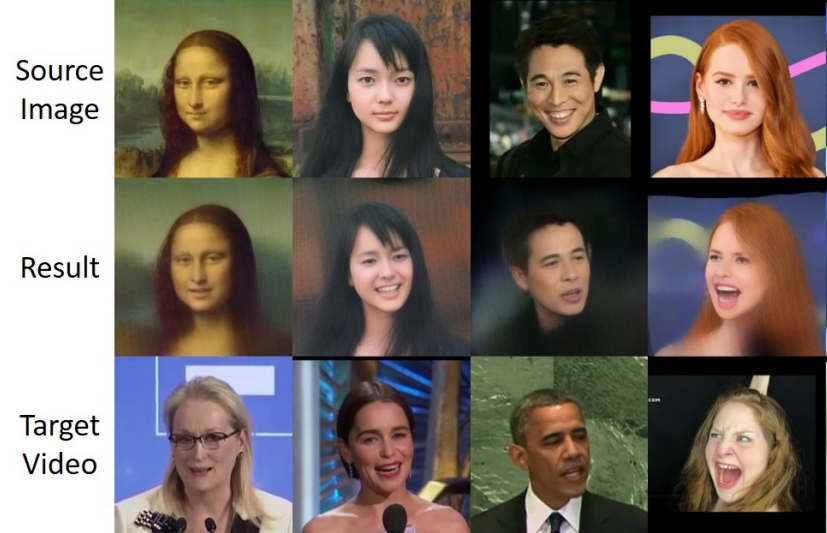
\includegraphics[width=0.7\textwidth]{Bilder/Reenactment}
    \centering
    \caption{Reenactment Ergebnisse eines \gls{fsgan}\cite{face-swapping-and-reenactment}}
    \label{fig:reenactment-fsgan}
\end{figure}

\subsubsection*{Full body puppetry}
Die letzte Art von Video Deepfakes ist die Full body puppetry, bei der einzelne Bewegungen bis hinzu komplette
Bewegungsabläufe auf eine andere Person übertragen werden.\newline
Die meisten Deepfakes benötigen viel Zeit für die Erstellung aufgrund der Systeme, welche erst mit dem Ausgangsmaterial trainiert werden müssen, um danach Inhalte verändern zu können.
Es gibt aber auch Deepfake-Methoden die in Echtzeit funktionieren, welche die Möglichkeit bietet, Mimik und Lippenbewegungen einer Person zu erkennen und diese anschließend in Echtzeit auf das Videobild einer anderen Person übertragen zu lassen.\cite{ResearchGate}

\subsubsection*{Audio Deepfakes}
Eine andere Art von Deepfakes sind Audio Deepfakes, bei dem aufgenommene oder live Audio Dateien verändert werden. Wobei hier zwischen Voice Swapping und Text to Speech unterschieden wird.\cite{ResearchGate}

\subsubsection*{Voice-swapping}
Bei dem Voice-swapping können Audioinhalte so verändert werden, dass ein Text von einer fremden Person gesprochen werden kann. Die Stimme kann mit verschiedenen Effekten verändert werden, sodass zum Beispiel eine Stimme jünger, älter, männlich, weiblich oder auch mit verschiedenen Dialekten versehen werden kann.
Dadurch wird dem Höhrer vorgespielt, dass verschiedene Personen sprechen, wobei es sich aber nur um eine Person hält.\cite{ResearchGate}

\subsubsection*{Text to Speech}
Beim Text to Speech können Audioinhalte einer Aufnahme durch Eingabe eines neuen Textes verändert werden. Dadurch können zum Beispiel falsch ausgesprochene Wörter im nachhinein ersetzt werden, ohne eine neue Aufnahme durchführen zu müssen.\cite{ResearchGate}

\subsubsection*{Foto Deepfakes}
Die dritte Art der Deepfakes sind Foto Deepfakes, bei denen es sich darum handelt, Fotos zu manipulieren. Dadurch können Fotos nach belieben verändert werden, um beispielsweise eine Person auf dem Bild durch einen Alterungsfilter, den Alterungsprozess der Person dargestellt werden kann.\cite{ResearchGate}

\subsubsection*{Face and body-swapping}
Mithilfe des Deepfake-Algorithmus, welcher auch bei den anderen Arten verwendet wird, können Änderungen an einem Gesicht und Körper gemacht werden, indem das Gesicht oder der Körper mit einer anderen Person ausgetauscht wird. Eine mögliche Anwendung hierfür wäre das virtuelle anprobieren einer Brille, Haarfarbe oder Kleidung.\cite{ResearchGate}

\subsubsection*{Kombination aus Audio und Video Deepfake}
Zuletzt gibt es wie oben eine mögliche Kombination der verschiedenen Arten, wie zum Beispiel die Kombination aus Audio und Video Deepfake.
Diese Kombination wird auch das Lip-syncing genannt, bei dem Mundbewegungen sowie die gesprochenen Wörter in einem Video verändert und synchronisiert werden.
Dadurch ist es möglich eine Person in einem Video scheinbar etwas sagen zu lassen, was sie aber niemals gesagt hat. Dies kann sowohl stark Missbraucht werden, indem zum Beispiel einem Politiker eine falschaussage untergeschoben wird.
Es kann aber auch für positive Sachen Verwendung finden, um beispielsweise einen Film oder Werbung in eine andere Sprache zu synchronisieren.\cite{ResearchGate}

\subsection{Anwendungsgebiete}
\subsubsection*{Positive Anwendungsgebiete}
Deepfakes können in den künstlerischen, satirischen, pädagogischen und sozialen Bereich positiv verwendet werden.\newline
So war es zum Beispiel möglich durch Deepfake-Technologien bekannte Persönlichkeiten wie Albert Einstein oder die Mona Lisa wieder zum Leben zu erwecken. Damit ist gemeint, dass so die bekannten Persönlichkeiten als Videos erstellt werden und dadurch besser in den Kontext gestellt werden können, um ein bestimmtes Thema in der Schule oder im Studium anschaulicher darstellen zu können.\newline
Es gibt auch zahlreiche Anwendungen von Deepfake in der Filmbranche, wie z.B. den Schauspieler mit dem Stunt double auszutauschen, verstorbene Schauspieler nochmals darstellen zu lassen oder auch bei der Synchronisation von verschiedenen Sprachen und den Mundbewegungen der Schauspieler.
Auch für Modeunternehmen sind Deepfake Technologien hilfreich, so kann der potenzielle Kunde zum Beispiel online bereits die Kleidung virtuell anprobieren und dann entscheiden, ob es ihm gefällt oder nicht.\newline
Künstlich generierte Gesichter wird auch als Alternative zur Unkenntlichmachung eingesetzt, um Privatsphäre und persönliche Daten (z.B. vor biometrischer Identifizierung) zu schützen.\newline
Text-To-Speech als Deepfakes sind sehr hilfreich, um Personen die ihre Sprachfähigkeit verloren haben durch einer Krankheit, kann so ihre Stimme zurückgegeben werden. Hierfür wird aus gesprochenen Sätzen der Person ein digitaler Klon der Stimme erstellt. So kann ein Computer dann eingegebene Texte mit der synthetisierten Stimme der erkrankten Person ausgeben.\cite{SpringerLink}

\subsubsection*{Negative Anwendungsgebiete}
Genauso wie es positive Anwendungsgebiete gibt, existieren natürlich auch einige negative Anwendungsbereiche für Deepfakes.
\begin{itemize}
    \item \textbf{Politik und Regierung:} \\
    Gerade in der Politik und Regierung Ebene können Deepfakes als Propaganda genutzt werden oder auch um Politiker in Videos oder Bilder falsch dazustellen und so Wahlen manipuliert werden. Dadurch entsteht bei der Regierung die Angst, dass Deepfakes eine Gefahr für die Demokratie sein könnte.\cite{ResearchGate}\newline Auch Diplomatische Beziehungen können negativ beeinflusst werden, so wurde zum Beispiel Deepfake-Videos vom ukrainischen und russischen Präsidenten veröffentlicht, indem der ukrainische Präsident zur Kapitualtion vor den Angriffen Russlands aufruft und der russische Präsident behauptet der Krieg sei beendet und es wäre Frieden zwischen beiden Ländern. Eine solche Fake Information, welche durch die Deepfakes sehr realisitsch erscheint, kann zu weitreichenden Konsequenzen auf der ganzen Welt führen. Auch gefälschte Videos von Soldaten oder Polizisten die unbewaffnete Zivilisten erschießen oder eine Ankündigung einer Katastrophe, wie z.B. einen Raketenangriff, kann zum Ausbruch von Protesten, Gewalt oder Massenpanik führen.\cite{SpringerLink}
    \item \textbf{Wirtschaft:} \\
    Deepfakes können auch Privatpersonen und Unternehmen schädigen, indem Sie Erpresst werden und zum Beispiel eine Entführung vortäuschen, um so Lösegeld zu fordern, ohne dass das vermeintliche Opfer sich in der Gewalt des Erpresser befindet.\newline Auch CEO-Frauds, bei denen dem Mitarbeiter eines Unternehmens vorgegaukelt wird, dass eine Führungsperson eine Überweisung eines hohen Geldbetrags oder ähnliches verlangt, werden immer realistischer. Darüber hinaus können Synthetische Medien auch zur Sabotage anderer Personen eingesetzt werden, um so ihren privaten und auch beruflichen Werdegang zu schädigen und dadurch sich zukünftige Geschäftschance nicht ergeben.\cite{SpringerLink}
    \item \textbf{Erstellung künstlicher Identitäten:} \\
    Durch den Einsatz realistischer synthetischer Fotos können künstliche Identitäten, die real nicht existieren und komplett künstlich erzeugt wurden, so glaubhaft dargestellt werden, dass diese für Authentifizierungsverfahren oder Spear Phishing Operationen eingesetzt werden können. Dadurch werden massenhafte Fake Profile auf Social Media erstellt, um andere User in Bezug auf private oder politischen Inhalte zu täuschen.\cite{SpringerLink}
    \item \textbf{Mobbing:} \\
    Auch Mobbing wird durch Deepfakes mehr Möglichkeiten gegeben, da jeder Mensch so leicht wie noch nie in lächerliche, gefährliche oder kompromittierende Szenarien gebracht werden kann.\cite{ResearchGate}
\end{itemize}

\subsection{Ethik}

Die Entwicklung von Deepfakes hat eine erhebliche Auswirkung auf die gesamte Welt. Deepfakes werden aus den verschiedensten Gründen verwendet, sei es für den Tausch von Gesichtern oder für eine Änderung von Stimmen.\newline
Was jedoch besonders beunruhigend daran ist, ist die Erstellung und Verbreitung von realistischen Fake News. Es wurde festgestellt, dass im Hinblick auf die ethischen Verpflichtungen dieser Technologie, Deepfake trotz der positiven Anwendungsbereiche überwiegend für bösartige Aktivitäten genutzt wird.\newline
Ein großes ethisches Problem im Zusammenhang mit Deepfake, ist die Verletzung der Privatsphäre. Nahezu jede digitale menschliche Spur kann gefälscht werden, was zu einer Bedrohung für die Privatsphäre führt. Ein weiterer Punkt ist die Zuverlässigkeit der Nachrichtensender, da die ausgestrahlten Nachrichten verfälscht sein könnten und alle Informationen in Frage gestellt werden, ob sie nun der Wahrheit entsprechen oder nicht.\newline
Dadurch hat sich die größte ethische Herausforderung gebildet im Zusammenhang mit Deepfakes. Diese Herausforderung besteht darin, dass schädliche Aktivitäten, wie die Fälschung und Verbreitung von gefälschten Informationen, immer häufiger werden und negative Auswirkungen auf die Gesellschaft haben.\newline
Auch Arbeitnehmer können sich in unethische Praktiken begeben, wie zum Beispiel die Entwicklung gefälschter Fotos und Videos eines Kollegen zu Unterhaltungs- oder Rachezwecken. Deshalb erfordert es eine kontinuierliche Bewertung der ethischen Aspekte des Arbeitsplatzes, um solche Taten zu umgehen.
Es wurde unter anderem festgestellt, dass die Nutzer durch der Entwicklung des Internets, leichten Zugang zu den Erstellungen von Deepfakes und dessen erforderlichen Werkzeugen erhalten. Das führt dazu, dass kein System, weder technologisch noch rechtlich,die Verwendung von Deepfakes stoppen kann, und dass aus ethischer und moralischer Sicht ein kontinuierlicher Schaden zu erwarten ist.\cite{Jatit}